%%
%% This is file `sample-acmsmall-conf.tex',
%% generated with the docstrip utility.
%%
%% The original source files were:
%%
%% samples.dtx  (with options: `acmsmall-conf')
%% 
%% IMPORTANT NOTICE:
%% 
%% For the copyright see the source file.
%% 
%% Any modified versions of this file must be renamed
%% with new filenames distinct from sample-acmsmall-conf.tex.
%% 
%% For distribution of the original source see the terms
%% for copying and modification in the file samples.dtx.
%% 
%% This generated file may be distributed as long as the
%% original source files, as listed above, are part of the
%% same distribution. (The sources need not necessarily be
%% in the same archive or directory.)
%%
%%
%% Commands for TeXCount
%TC:macro \cite [option:text,text]
%TC:macro \citep [option:text,text]
%TC:macro \citet [option:text,text]
%TC:envir table 0 1
%TC:envir table* 0 1
%TC:envir tabular [ignore] word
%TC:envir displaymath 0 word
%TC:envir math 0 word
%TC:envir comment 0 0
%%
%%
%% The first command in your LaTeX source must be the \documentclass command.
\documentclass[acmsmall, screen]{acmart}

%%
%% \BibTeX command to typeset BibTeX logo in the docs
\AtBeginDocument{%
  \providecommand\BibTeX{{%
    \normalfont B\kern-0.5em{\scshape i\kern-0.25em b}\kern-0.8em\TeX}}}

%% Rights management information.  This information is sent to you
%% when you complete the rights form.  These commands have SAMPLE
%% values in them; it is your responsibility as an author to replace
%% the commands and values with those provided to you when you
%% complete the rights form.
%\setcopyright{acmcopyright}
%\copyrightyear{2018}
%\acmYear{2018}
%\acmDOI{10.1145/1122445.1122456}

%% These commands are for a PROCEEDINGS abstract or paper.
%\acmConference[Woodstock '18]{Woodstock '18: ACM Symposium on Neural
%  Gaze Detection}{June 03--05, 2018}{Woodstock, NY}
%\acmBooktitle{Woodstock '18: ACM Symposium on Neural Gaze Detection,
%  June 03--05, 2018, Woodstock, NY}
%\acmPrice{15.00}
%\acmISBN{978-1-4503-XXXX-X/18/06}


%%
%% Submission ID.
%% Use this when submitting an article to a sponsored event. You'll
%% receive a unique submission ID from the organizers
%% of the event, and this ID should be used as the parameter to this command.
%% \acmSubmissionID{123-A56-BU3}

%%
%% The majority of ACM publications use numbered citations and
%% references.  The command \citestyle{authoryear} switches to the
%% "author year" style.
%%
%% If you are preparing content for an event
%% sponsored by ACM SIGGRAPH, you must use the "author year" style of
%% citations and references.
%% Uncommenting
%% the next command will enable that style.
%%\citestyle{acmauthoryear}
\usepackage{import}
\usepackage{xifthen}
\usepackage{pdfpages}
\usepackage{transparent}
\newcommand{\incfig}[1]{%
    \def\svgwidth{\columnwidth}
    \import{./img/}{#1.pdf_tex}
}
%%
%% end of the preamble, start of the body of the document source.
\begin{document}

%%
%% The "title" command has an optional parameter,
%% allowing the author to define a "short title" to be used in page headers.
\title{The Name of the Title is Hope}

%%
%% The "author" command and its associated commands are used to define
%% the authors and their affiliations.
%% Of note is the shared affiliation of the first two authors, and the
%% "authornote" and "authornotemark" commands
%% used to denote shared contribution to the research.
\author{Yanjun Chen}
\authornote{Research advisor: Cyrus Omar}
\email{yanjunc@umich.edu}
%\orcid{1234-5678-9012}
\authornotemark[1]
\affiliation{%
  \institution{University of Michigan}
  %\streetaddress{P.O. Box 1212}
  %\city{Dublin}
  %\state{Ohio}
  \country{USA}
  %\postcode{43017-6221}
}

%%
%% By default, the full list of authors will be used in the page
%% headers. Often, this list is too long, and will overlap
%% other information printed in the page headers. This command allows
%% the author to define a more concise list
%% of authors' names for this purpose.
\renewcommand{\shortauthors}{Trovato and Tobin, et al.}

%%
%% The abstract is a short summary of the work to be presented in the
%% article.
% \begin{abstract}
%   A clear and well-documented \LaTeX\ document is presented as an
%   article formatted for publication by ACM in a conference proceedings
%   or journal publication. Based on the ``acmart'' document class, this
%   article presents and explains many of the common variations, as well
%   as many of the formatting elements an author may use in the
%   preparation of the documentation of their work.
% \end{abstract}

%%
%% The code below is generated by the tool at http://dl.acm.org/ccs.cfm.
%% Please copy and paste the code instead of the example below.
%%
%TODO: I don't know what it is.
% \begin{CCSXML}
% <ccs2012>
%  <concept>
%   <concept_id>10010520.10010553.10010562</concept_id>
%   <concept_desc>Computer systems organization~Embedded systems</concept_desc>
%   <concept_significance>500</concept_significance>
%  </concept>
%  <concept>
%   <concept_id>10010520.10010575.10010755</concept_id>
%   <concept_desc>Computer systems organization~Redundancy</concept_desc>
%   <concept_significance>300</concept_significance>
%  </concept>
%  <concept>
%   <concept_id>10010520.10010553.10010554</concept_id>
%   <concept_desc>Computer systems organization~Robotics</concept_desc>
%   <concept_significance>100</concept_significance>
%  </concept>
%  <concept>
%   <concept_id>10003033.10003083.10003095</concept_id>
%   <concept_desc>Networks~Network reliability</concept_desc>
%   <concept_significance>100</concept_significance>
%  </concept>
% </ccs2012>
% \end{CCSXML}

% \ccsdesc[500]{Computer systems organization~Embedded systems}
% \ccsdesc[300]{Computer systems organization~Redundancy}
% \ccsdesc{Computer systems organization~Robotics}
% \ccsdesc[100]{Networks~Network reliability}

%%
%% Keywords. The author(s) should pick words that accurately describe
%% the work being presented. Separate the keywords with commas.
% \keywords{datasets, neural networks, gaze detection, text tagging}

%% A "teaser" image appears between the author and affiliation
%% information and the body of the document, and typically spans the
%% page.
% \begin{teaserfigure}
%   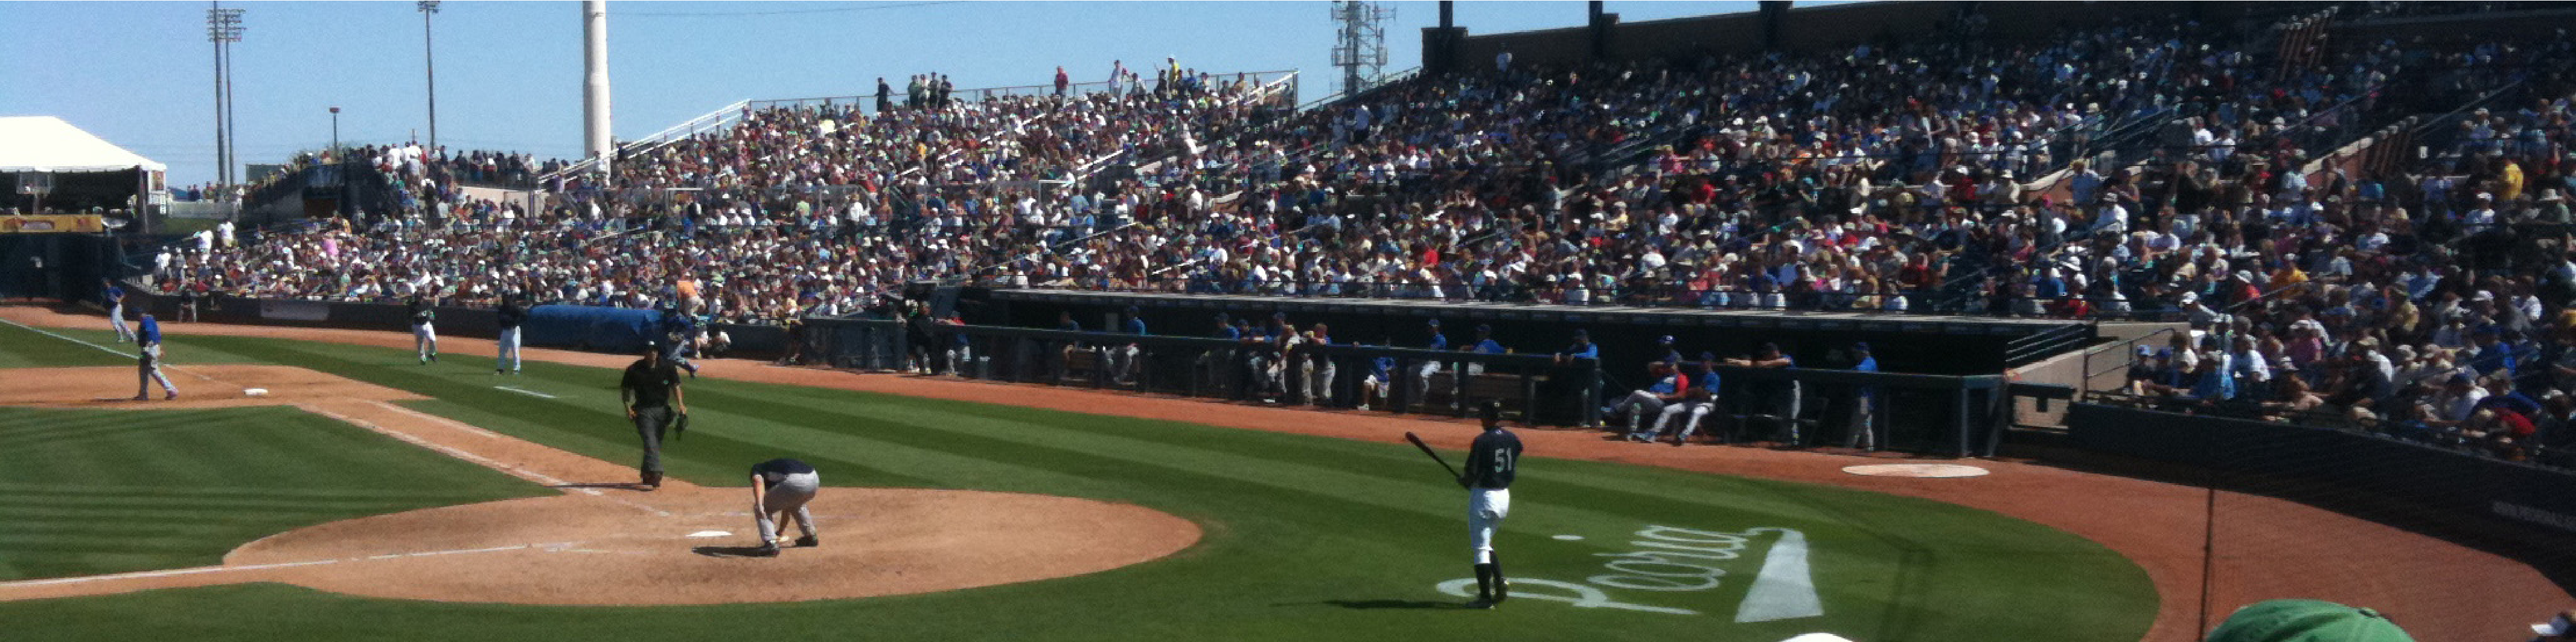
\includegraphics[width=\textwidth]{sampleteaser}
%   \caption{Seattle Mariners at Spring Training, 2010.}
%   \Description{Enjoying the baseball game from the third-base
%   seats. Ichiro Suzuki preparing to bat.}
%   \label{fig:teaser}
% \end{teaserfigure}

%%
%% This command processes the author and affiliation and title
%% information and builds the first part of the formatted document.
\maketitle





% \section{Acknowledgments}

% Identification of funding sources and other support, and thanks to
% individuals and groups that assisted in the research and the
% preparation of the work should be included in an acknowledgment
% section, which is placed just before the reference section in your
% document.

% This section has a special environment:
% \begin{verbatim}
%   \begin{acks}
%   ...
%   \end{acks}
% \end{verbatim}
% so that the information contained therein can be more easily collected
% during the article metadata extraction phase, and to ensure
% consistency in the spelling of the section heading.

% Authors should not prepare this section as a numbered or unnumbered {\verb|\section|}; please use the ``{\verb|acks|}'' environment.

% \section{Appendices}

% If your work needs an appendix, add it before the
% ``\verb|\end{document}|'' command at the conclusion of your source
% document.

% Start the appendix with the ``\verb|appendix|'' command:
% \begin{verbatim}
%   \appendix
% \end{verbatim}
% and note that in the appendix, sections are lettered, not
% numbered. This document has two appendices, demonstrating the section
% and subsection identification method.

% \section{SIGCHI Extended Abstracts}

% The ``\verb|sigchi-a|'' template style (available only in \LaTeX\ and
% not in Word) produces a landscape-orientation formatted article, with
% a wide left margin. Three environments are available for use with the
% ``\verb|sigchi-a|'' template style, and produce formatted output in
% the margin:
% \begin{itemize}
% \item {\verb|sidebar|}:  Place formatted text in the margin.
% \item {\verb|marginfigure|}: Place a figure in the margin.
% \item {\verb|margintable|}: Place a table in the margin.
% \end{itemize}

%%
%% The acknowledgments section is defined using the "acks" environment
%% (and NOT an unnumbered section). This ensures the proper
%% identification of the section in the article metadata, and the
%% consistent spelling of the heading.
% \begin{acks}
% To Robert, for the bagels and explaining CMYK and color spaces.
% \end{acks}

%%
%% The next two lines define the bibliography style to be used, and
%% the bibliography file.
\bibliographystyle{ACM-Reference-Format}
\bibliography{sample-base}

%%
%% If your work has an appendix, this is the place to put it.
% \appendix

% \section{Research Methods}

% \subsection{Part One}

% Lorem ipsum dolor sit amet


\end{document}
\endinput
%%
%% End of file `sample-acmsmall-conf.tex'.
